\begin{frame}[plain,c]
	\begin{center}
		\huge Representation \\
		\small of STS(v)
	\end{center}
\end{frame}

\begin{frame}
	\frametitle{How to represent}
	\begin{columns}
		\column{0.5\textwidth}
		\begin{itemize}
			\item through display each 3-set of $T$ and $S$ ($\{a,b,c,d,e,f,g\}$,$\{$\\ $\{a,b,c\},\{b,d,e\},...,\{d,f,g\}\}$)
			\item through a \textit{\textcolor{red}{complete} graph}
		\end{itemize}
		\column{0.5\textwidth}
		\begin{figure}
			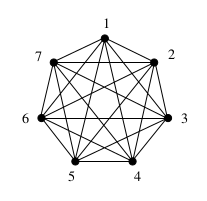
\includegraphics[scale=0.5]{complete_graph}
			\caption{A complete graph of order $v=7$}
		\end{figure}
	\end{columns}
\end{frame}

\begin{frame}
	\frametitle{Example}
	Why a focus on representation?
	\begin{itemize}
		\item we talk about combinatorial design (display somehow somethings)
		\item help to design algorithm
	\end{itemize}
	
	\begin{figure}
		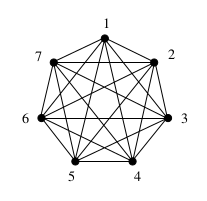
\includegraphics[scale=0.5]{complete_graph}
		\caption{A complete graph of order $v=7$}
	\end{figure}

	%possiamo pensare a qualche modo per ragionare meglio sugli sts?
	\pause

	\setbeamercolor{block title}{bg=red!30,fg=blue}
	\begin{block}{Focus on}
		How to choose a proper partition of the graph ? 
	\end{block}
\end{frame}

%these show that intuition, sometimes, may be an option
\begin{frame}
\frametitle{Example}
First non-dummy: STS of \textit{order} $7$
\begin{columns}
	\column{0.5\textwidth}
	\begin{figure}
		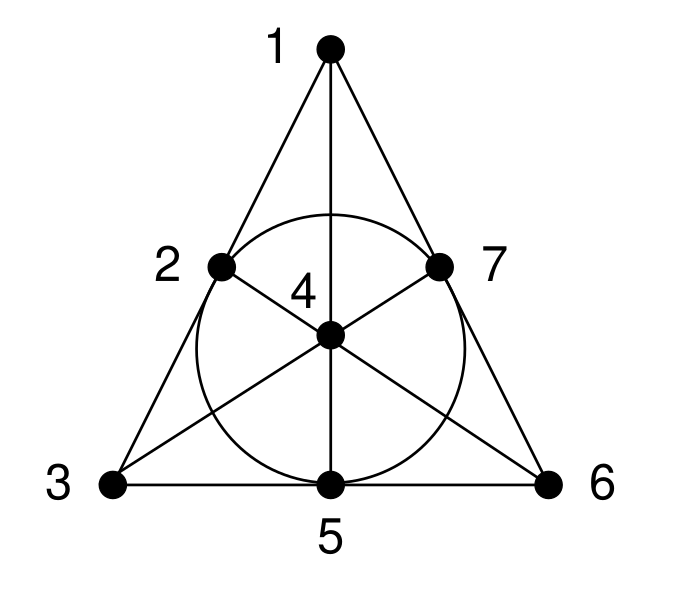
\includegraphics[width=0.7\textwidth]{fano_plane}
		\caption{Fano plane}
	\end{figure}
	\column{0.5\textwidth}
	\begin{figure}
		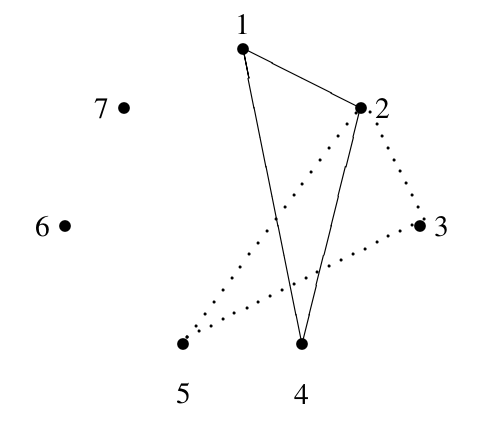
\includegraphics[width=0.7\textwidth]{triangle_on_sts_7}
		\caption{Building methods on STS($7$)}
	\end{figure}
\end{columns}
\end{frame}